\documentclass[conference]{IEEEtran}

\usepackage{amsmath,amssymb,amsfonts}
\usepackage{graphicx}
\usepackage{cite}
\usepackage{hyperref}
\usepackage{booktabs}
\usepackage{multirow}

\title{LibRec: Comparing Social-Aware Recommender Systems}

\author{
  \IEEEauthorblockN{Cale Smith, Advait Shinde, Jasper Morgal}
  \IEEEauthorblockA{Department of Computer Engineering\\
  San Jose State University\\
  San Jose, CA, USA\\
  \{cale.smith, advait.shinde, jasper.morgal\}@sjsu.edu}
}

\begin{document}

\maketitle

\begin{abstract}
Recommender systems have a tendency to struggle with sparse ratings, especially 
in cold-start settings. In this project we attempt to beat simple baselines by 
leveraging trust graphs. To do this we use the LibraryThing dataset (1.7M 
reviews and 83K users) which contains the classic (user, item, rating) tuple as 
well as a trust graph. We build a shared pipeline along with two baselines, a 
global mean and an untuned LightGBM model, and then attempt to beat those 
baselines across rating-accuracy and ranking-quality metrics. To do this we 
implement Three models, a hyper-tuned LightGBM model, a Neural Collaborative 
Filtering (NCF) model with social regularization, and a Graph Convolution over 
the user-item interaction graph.
\end{abstract}

\noindent\textbf{Repository:} \url{https://www.github.com/calepayson/librec}

\section{Introduction}
\label{sec:intro}

Collaborative filtering (CF) is one of the fundamental strategies of 
recommender systems but, despite improvements, still struggles with sparse 
user-item interaction matrices. Our chosen dataset, LibraryThing, is incredibly
sparse, with only 0.0041\% of user-item combinations being filled in. 
Compounding the difficulty, only 38\% of users have rated more than five items.

While this would make standard collaborative filtering approaches quite
unreliable, LibraryThing also includes other metadata, the most important
addition being a friendship graph (with 219K edges). This social signal gives 
us the opportunity to test social-aware recommender systems against classic 
baselines. With that in mind our goal is to see how various strategies perform
against the baseline.

We test this with a comparative study. We create a shared pipeline that ensures
each model shares the same preprocessing step and is evaluated on the same
metrics. The models are as follows:

\begin{itemize}
  \item \textbf{Variant A}: (Baseline): Global Mean - Simply returns the average rating of the training set.
  \item \textbf{Variant B}: (Baseline): Untuned-LightGBM - A LightGBM model with default hyperparameters.
  \item \textbf{Variant C} (Jasper): Hyper-tuned LightGBM - Takes the baseline and evaluates the performance difference of aggressive hyperparameter tuning.
  \item \textbf{Variant D} (Cale): SocialNCF - Combines neural collaborative filtering (NCF) with social graph regularization and neighbor-averaging cold-start inference.
  \item \textbf{Variant E} (Advait): Graph Convolutional Network over the user-item interaction graph.
\end{itemize}

\section{Dataset Analysis}
\label{sec:data}

We use the LibraryThing dataset from the McAuley Lab collection~\cite{koren2009mf}, which pairs user--item ratings with a social friendship graph. Table~\ref{tab:datasets} summarizes its key statistics.

\begin{table}[htbp]
\caption{LibraryThing Dataset Statistics}
\label{tab:datasets}
\centering
\begin{tabular}{lr}
\toprule
\textbf{Metric} & \textbf{Value} \\
\midrule
Reviews          & 1,707,070 \\
Users            & 83,195    \\
Items            & 506,165   \\
Social edges     & 219,790   \\
Sparsity (\%)    & 0.0041    \\
Users $\leq$5 ratings (\%) & 62.0 \\
Users in social graph (\%) & 30.8 \\
Cold users w/ social (\%)  & 21.5 \\
User Gini        & 0.809     \\
Item Gini        & 0.632     \\
Mean rating      & 3.81      \\
Rating std       & 1.00      \\
\bottomrule
\end{tabular}
\end{table}

\begin{figure}[htbp]
\centering
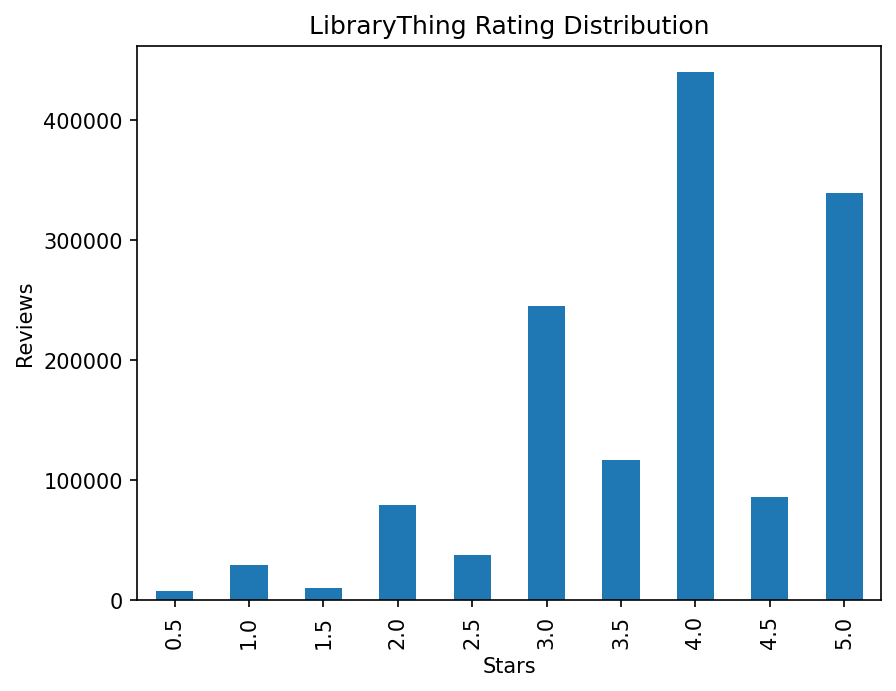
\includegraphics[width=\columnwidth]{lthing_ratings.png}
\caption{LibraryThing rating distribution.}
\label{fig:lthing-ratings}
\end{figure}

LibraryThing is a book review platform with 1.7M ratings from 83K users across 
506K works. Ratings use a half-star scale (0.5-5.0) and peak at 4.0 stars
(Figure~\ref{fig:lthing-ratings}), suggesting that users tend to rate books 
they enjoyed. The user activity distribution is highly unequal (Gini = 0.809), 
a small core of power users contributes disproportionately, while 62\% of users 
have five or fewer ratings. The social friendship graph covers 30.8\% of users, 
and among cold-start users ($\leq$5 ratings), 21.5\% have at least one social 
connection which provides a meaningful signal for social-aware methods.

\section{Shared Pipeline and Baselines}
\label{sec:pipeline}

Our pipeline uses a modular structure where each module produces a cached 
artifact that following stages can use. This makes it easy to collaborate on 
the project without having having to rebuild the entire pipeline on every 
change.

\subsection{Preprocessing}

We process the raw data in a few steps, each of which produces a cached
artifact. First we convert the raw review data into the standard (user, item, 
rating) format, although we also include a time feature. We then use the time
feature to apply temporal 80/10/10 split, where the train set has the oldest
80\% of data, the val set has the next oldest 10\%, etc.

After splitting the data we transform it. First, user and item identifiers are
encoded as integers using the training set identifiers. Users or items that 
don't appear in the training set (cold-start) are given a value of -1 though 
we also extend the codes for socially aware models. Second, we normalize the 
user ratings per user. Third, we update the temporal feature to reflect time
since the first datapoint rather than unix time. 

We also update the LibraryThing friendship graph to reflect the new user
encodings, discarding any users who aren't included in the training data.

\subsection{Evaluation Framework}

All models are evaluated using the same framework implemented in a shared 
BaseModel class. This BaseModel presents a shared interface to be used by each
model and computes two classes of metrics:

\textbf{Rating accuracy:} Root Mean Squared Error (RMSE) and Mean Absolute 
Error (MAE), computed on both validation and test sets. These measure how well 
a model predicts the exact star rating a user would assign.

\textbf{Ranking quality:} Precision@10, Recall@10, NDCG@10, and Hit Rate@10. 
For these, we define a rating $\geq 4.0$ as ``relevant.'' For each user, we 
take the top 10 items by predicted score and compute precision (fraction of 
top-10 that are relevant), recall (fraction of all relevant items captured in 
top-10), NDCG (position-weighted relevance), and hit rate (whether at least one 
relevant item appears in top-10).

\subsection{Baseline: Global Mean}

Our simplest baseline predicts the training-set mean rating (3.81) for every 
user-item pair. This model is trivial but establishes a floor: any method that 
cannot beat global mean is not learning useful patterns from the data.

\subsection{Baseline: LightGBM}

Our second baseline is a LightGBM~\cite{ke2017lightgbm} gradient-boosted 
decision tree regressor. It takes a user code and an item code as categorical 
input features and predicts the rating. Training uses 500 boosting rounds with 
early stopping on validation RMSE. Key hyperparameters include 63 leaves per 
tree, learning rate 0.05, and 90\% feature/bagging fractions. Unseen users and 
items in the validation and test sets receive code -1, which LightGBM treats as 
a distinct category. This baseline is substantially stronger than global mean, 
as it can learn per-user and per-item biases.

\section{Hyper-Tuned LightGBM}
\label{sec:tuned-lgbm}

\textit{Jasper Morgal}

\subsection{Design and Motivation}

TODO

\subsection{Implementation Details}

TODO

\subsection{Design Decision Log}

\begin{table}[htbp]
\caption{Hyper-Tuned LightGBM --- Key Design Decisions}
\label{tab:decisions-tuned-lgbm}
\centering
\begin{tabular}{p{2.5cm}p{2.5cm}p{2.5cm}}
\toprule
\textbf{Choice} & \textbf{Selected} & \textbf{Alternatives} \\
\midrule
TODO & TODO & TODO \\
\bottomrule
\end{tabular}
\end{table}

\subsection{Results and Analysis}

TODO

\section{SocialNCF}
\label{sec:social-ncf}

\textit{Cale Smith}

\subsection{Design and Motivation}

The LightGBM baselines treat user and item codes as categorical features, 
learning per-entity biases but not dense interactions. Neural Collaborative 
Filtering (NCF)~\cite{he2017ncf} addresses this by learning dense embedding 
vectors for each user and item and combining them through both linear (GMF) and 
nonlinear (MLP) pathways. Also, I like deep learning and just wanted to add a
neural net.

However, NCF learns embeddings just from rating interactions. Since our 
exploratory data analysis shows that 21.5\% of cold-start LibraryThing users 
have social connections, I wondered if the rating could be improved with that 
info. Social-Regularized NCF extends NCF by incorporating the social graph in 
two ways:

\begin{enumerate}
  \item \textbf{Training-time regularization:} A penalty term encourages the GMF embeddings of socially connected users to be similar. I based this off of Ma et al.~\cite{ma2011soreg}.
  \item \textbf{Cold-start inference:} For users with no training ratings but at least one social connection, I used the mean of their freinds' embeddings (both GMF and MLP).
\end{enumerate}

\subsection{Implementation Details}

I implemented the NeuMF architecture based on He et al.~\cite{he2017ncf}. The 
model has four embeddings: user and item embeddings for the GMF path, 
and user and item embeddings for the MLP path, each with 32 dimensions (kept it 
at 32 because my computer is a potato). The GMF path computes element-wise 
products of user and item embeddings. The MLP path concatenates user and item 
embeddings (64-dimensional input) and passes them through two hidden layers of 
size 64 and 32 with ReLU activations and 10\% dropout. The GMF output and MLP 
output are concatenated and fed to a linear prediction layer that produces the
final rating.

I used the Adam optimizer with a learning rate of $10^{-3}$, a batch size of
8192, and MSE loss. I used early stopping after 5
epochs of no improvement on the validation set. The linear layer weights were
initialized with Xavier uniform distribution and normal distribution for
embeddings.

The social regularization term is added to the loss at each training step:
\begin{equation}
  \mathcal{L} = \mathcal{L}_{\text{MSE}} + \lambda \cdot \frac{1}{|E|} \sum_{(u,v) \in E} \|\mathbf{p}_u - \mathbf{p}_v\|^2
\end{equation}
where $E$ is the set of trust/friendship edges between training-set users, 
$\mathbf{p}_u$ denotes the GMF embedding of user $u$, and $\lambda = 0.01$.

To handle cold-start users, the preprocessing pipeline assigns integer codes to 
all users: training users receive codes $0$ to $n_{\text{train}}-1$, while 
users in only validation/test receive codes $n_{\text{train}}$ and above. At 
inference time, a cold-start user $u$ with neighbor set $\mathcal{N}(u)$, is
computed with:
\begin{equation}
  \hat{\mathbf{p}}_u = \frac{1}{|\mathcal{N}(u)|} \sum_{v \in \mathcal{N}(u)} \mathbf{p}_v
\end{equation}
and same for the MLP embedding. These averaged embeddings are passed through 
the full NeuMF forward pass to produce predictions. Unseen users with no social
connections are just assigned the global average rating as a prediction.

\subsection{Design Decisions}

\begin{table}[htbp]
\caption{SocialNCF --- Key Design Decisions}
\label{tab:decisions-social-ncf}
\centering
\begin{tabular}{p{2.5cm}p{2.5cm}p{2.5cm}}
\toprule
\textbf{Choice} & \textbf{Selected} & \textbf{Alternatives Tried} \\
\midrule
Architecture & SocialNeuMF & NeuMF \\
Embedding dim & 32 & 64, 128 \\
Learning rate & $10^{-3}$ & $5\times10^{-4}$, $10^{-4}$ \\
Loss function & MSE & RMSE \\
Reg.\ target & GMF embeddings & None \\
$\lambda$ & 0.01 & 0.001, 0.1, 1.0 \\
Cold-start strategy & Social Mean & None \\
\bottomrule
\end{tabular}
\end{table}

\subsection{Results and Analysis}

The base NCF model (without social regularization) scored a test RMSE of 0.9922
and MAE of 0.7811, slightly worse than the untuned LightGBM baseline (RMSE
0.9690). Adding social regularization brought the test RMSE down marginally to
0.9919 and improved MAE to 0.7794. More notably, Social NCF improved ranking
metrics over base NCF: Precision@10 rose from 0.3045 to 0.3074 and NDCG@10
from 0.7379 to 0.7422. This suggests the social regularization term helps the
model learn embeddings that better capture user preference, even if the rating 
accuracy improvement is small.

The cold-start neighbor-averaging strategy allows Social NCF to produce
personalized predictions for users who have no training ratings but do have
friends in the graph. Without this, those users would just receive the global
mean prediction. 

But, all that being said, it didn't beat the simple LightGBM baseline, despite
many hours of hyperparameter tuning that I wish I could take back. Stick with
the simple model first kids. Complexity is tough.

\section{Graph Convolutional Network}
\label{sec:gcn}

\textit{Advait Shinde}

\subsection{Design and Motivation}

TODO

\subsection{Implementation Details}

TODO

\subsection{Design Decision Log}

\begin{table}[htbp]
\caption{GCN --- Key Design Decisions}
\label{tab:decisions-gcn}
\centering
\begin{tabular}{p{2.5cm}p{2.5cm}p{2.5cm}}
\toprule
\textbf{Choice} & \textbf{Selected} & \textbf{Alternatives} \\
\midrule
TODO & TODO & TODO \\
\bottomrule
\end{tabular}
\end{table}

\subsection{Results and Analysis}

TODO

\section{Comparative Analysis and Discussion}
\label{sec:comparison}

\begin{table*}[htbp]
\caption{Performance Comparison Across All Models (LibraryThing)}
\label{tab:results-lthing}
\centering
\begin{tabular}{lcccccc}
\toprule
\textbf{Model} & \textbf{Val RMSE} & \textbf{Test RMSE} & \textbf{Test MAE} & \textbf{P@10} & \textbf{R@10} & \textbf{NDCG@10} \\
\midrule
Global Mean      & 0.9956 & 0.9945 & 0.7852 & 0.2995 & 0.7237 & 0.7248 \\
LightGBM         & 0.9551 & 0.9690 & 0.7510 & 0.3115 & 0.7295 & 0.7491 \\
Tuned LightGBM   & TODO   & TODO   & TODO   & TODO   & TODO   & TODO   \\
NCF              & 0.9884 & 0.9922 & 0.7811 & 0.3045 & 0.7270 & 0.7379 \\
Social NCF       & 0.9916 & 0.9919 & 0.7794 & 0.3074 & 0.7283 & 0.7422 \\
GCN              & TODO   & TODO   & TODO   & TODO   & TODO   & TODO   \\
\bottomrule
\end{tabular}
\end{table*}

\subsection{Rating Prediction}

TODO

\subsection{Ranking Quality}

TODO

\subsection{Effect of Social Information}

TODO

\subsection{Ablation Studies}

TODO

\section{Individual Reflections}
\label{sec:reflections}

\subsection{Cale Smith}
I was not expecting to get destroyed by an untuned LightGBM. Damn. I think the
biggest reason is that this is a super sparse dataset, even whith the
friendship graph, and LightGBM is great at cold-start predictions. Because of
the sparsity of the dataset I was relying on global mean for a ton of my
predictions and the social regularization that I used just ran into the same
problem with an extra step. Instead of directly predicting mean it went through
a bunch of extra steps that, if we're being honest, basically ended up at the
same mean. We manipulated the embeddings so that friends were in similar vector
spaces but, because the graph is so sparse, we still ended up with predictions
that were still heavily reflective of the global mean. 

The implementation was super fun and I had a blast training it, though it felt
like there wasn't enough time to do everything I wanted within the project 
start/end window. In hindsight I think two things stand out. First, I'm going
to use the simplest model I can to start every future ML project, I really
suspect that it's an underated strategy with school projects. Second, I tried
to add a ton of regularization and to get a double descent situation but it 
just didn't work. I think this was because, while the dataset was massive I
didn't have enough complexity in my model (had to keep the layers and embeddings
pretty small so that it would run on my potato-ass laptop), and the sparsity
meant that there just wasn't much signal there in the first place.

All in all, sparsity sucks. The end.

\subsection{Advait Shinde}
TODO

\subsection{Jasper Morgal}
TODO

\section{Conclusion}
\label{sec:conclusion}

TODO

\bibliographystyle{IEEEtran}
\bibliography{references}

\end{document}
